\label{ch:appendixB}

\section{General Overview}

In the backward elimination method, we start with Eq. \ref{eq:greens_function2}, repeated here for convenience.
\begin{equation}\label{eq:greens_function2_back}
    \begin{aligned}
        \delta \phi(\textbf{r}, \omega) &= \sum_{\textbf{r}_p} G(\textbf{r}, \textbf{r}_p,\omega) S(\textbf{r}_p,\omega)
    \end{aligned}
\end{equation}
As seen in Eq. \ref{eq:greens_function2_back}, the neutron noise can be constructed as a finite combination of Green's function matrix and the noise source as the coefficient. This is a finite combination since there are $(\text{group} \times N)^{(\text{group} \times N)}$ possible combinations of solutions that are true in this problem. The backward elimination method starts with the assumption that the noise source is defined in every mesh of the problem. This will overfit the solution of reconstructed neutron noise. Then, for every iteration, the Green's function component that has the smallest contribution to the solution is eliminated. This process is repeated until it finds the smallest possible number of solutions that could pass the residual tolerance. By then, the combination that has the smallest number of components is the solution of the neutron noise vector.

The flow diagram of the method is described in Figure \ref{fig:backward_elimination_method}
\begin{figure}[H]
        \centering
        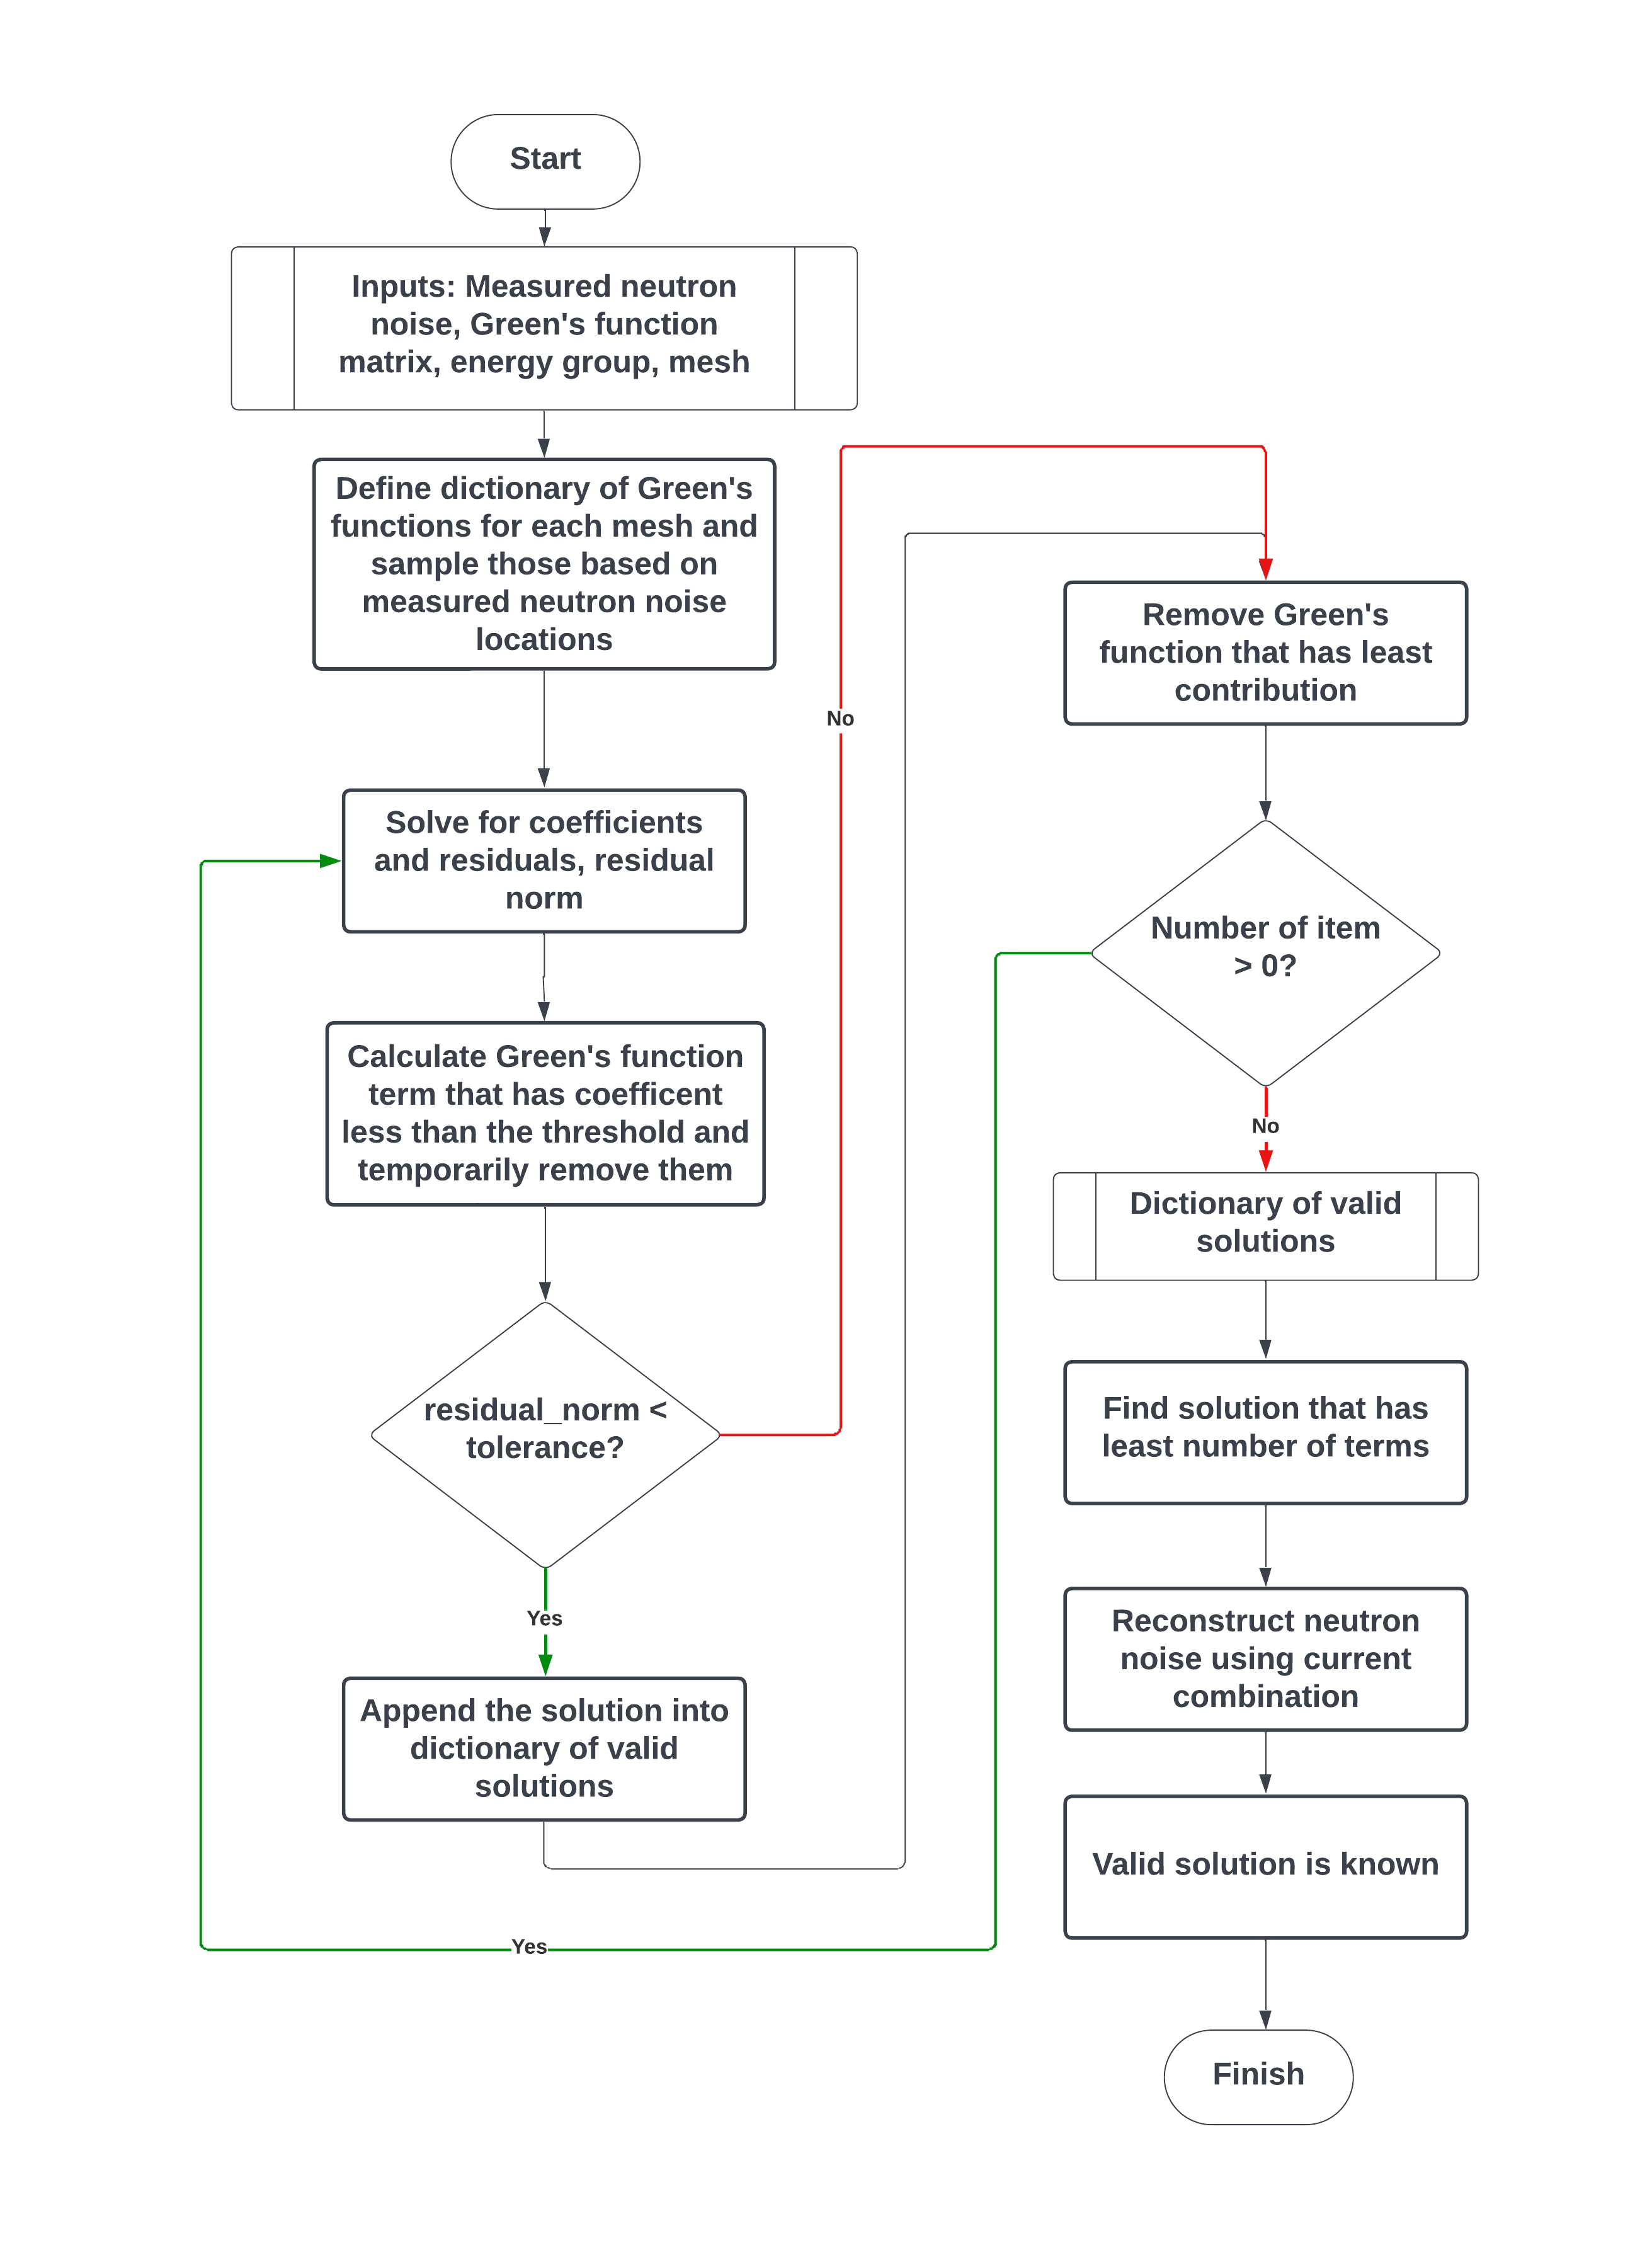
\includegraphics[width=0.6\textwidth]{figures/Backward Elimination.png}
        \caption{Flow diagram of backward elimination method}
        \label{fig:backward_elimination_method}
\end{figure}

The pseudo algorithm for the backward elimination method is described in Algorithm~\ref{alg:backward_unfold}
\begin{algorithm}[H]
\caption{: Backward Elimination Method}
\label{alg:backward_unfold}
\begin{algorithmic}[1]
\Require Measured neutron noise $\delta \phi(\textbf{r}_{\text{meas}}, \omega)$, Green’s function matrix $G(\textbf{r}, \textbf{r}_p,\omega)$, energy groups $g$, mesh $N$
\Ensure Reconstructed neutron noise $\delta \phi_{\text{BACK}}(\textbf{r}, \omega)$, unfolded source $S_{\text{BACK}}(\textbf{r}, \omega)$
\For{each group $g$} \Comment{\textbf{Construct Green’s function dictionary}}
    \For{each node $n$}
        \State Store column $G_{g,n}$ = column of $G(\textbf{r}, \textbf{r}_p,\omega)$ in a dictionary
    \EndFor
\EndFor
\State Sample columns only at measured (non-zero) indices
\State Initialize selected columns $\gets \{ \text{all columns} \}$
\While{selected columns $\neq \emptyset$} \Comment{\textbf{Iterative backward elimination}}
    \State Solve least-squares: $\mathbf{c} = \arg\min ||\delta \phi(\textbf{r}_{\text{meas}}, \omega) - A \mathbf{c}||$ with current columns
    \State Compute residual norm $||r||$
    \State Compute contributions of each column: $|c_i| / \max_j |c_j|$
    \If{$||r|| < \text{tolerance}$}
        \State Store current solution as valid
        \State Remove least contributing column and continue
    \Else
        \State Remove least contributing column
    \EndIf
\EndWhile

\If{no valid solution is found, }  \Comment{\textbf{Select best solution}}
    \State \Return failure
\Else
    \State Select best valid solution (fewest columns)
    \State Reconstruct flux: $\delta \phi_{\text{BACK}}(\textbf{r}, \omega) = \sum c_i G_{i}$
\EndIf
\State Solve $S_{\text{BACK}}(\textbf{r}, \omega) = G^{-1}(\textbf{r}, \textbf{r}_p,\omega) \delta \phi_\text{BACK}(\textbf{r}, \omega)$
\State \textbf{Postprocess:} $S_{\text{BACK}}(\textbf{r}, \omega)$ file, $\delta \phi_\text{BACK}(\textbf{r}, \omega)$ file, plots. 
\end{algorithmic}
\end{algorithm}

This method is applied to 2D HTTR problems similar to the problems in Section \ref{ch:unfolding_methods}. The results are described in the following section.

\section{Application of HTTR Core}

\subsection{2D HTTR with Absorber of Variable Strength Source}

\subsubsection{Single Noise Source}

In this simulation, single mesh AVS source is unfolded using both the existing and novel methods. The simulation is done with a constant frequency of 0.316 Hz. Figure \ref{fig:map_S_2DHTTR_AVS1S_back} shows the location of the AVS source.
\begin{figure}[H]
        \centering
        \begin{subfigure}{.48\textwidth}
          \centering
          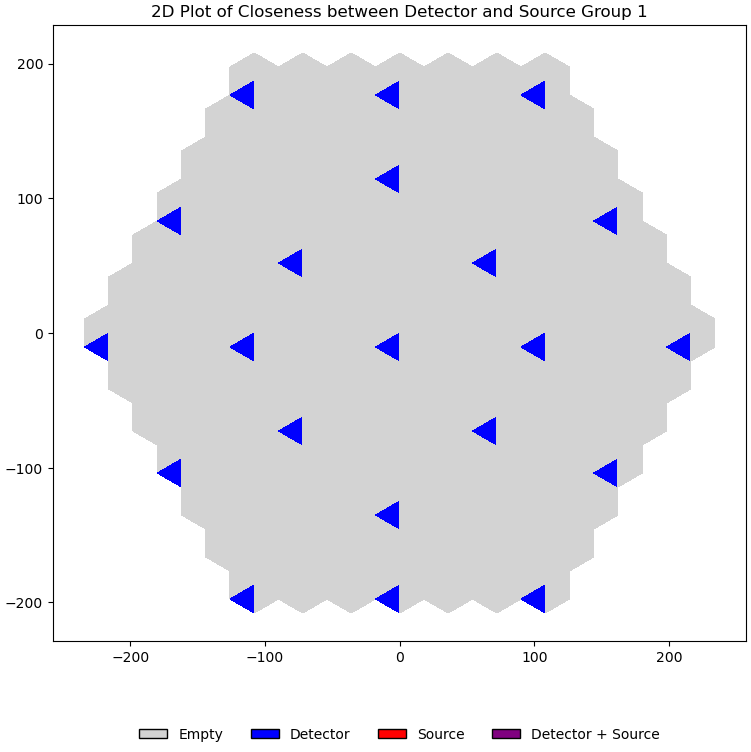
\includegraphics[width=\linewidth]{figures/OBJECTIVES61_TEST_SUITE_2DTriMG_HTTR_level1_iter2_closeness_det_S_categorical_G1.png}
        \end{subfigure}
        \hfill
        \begin{subfigure}{.48\textwidth}
          \centering
          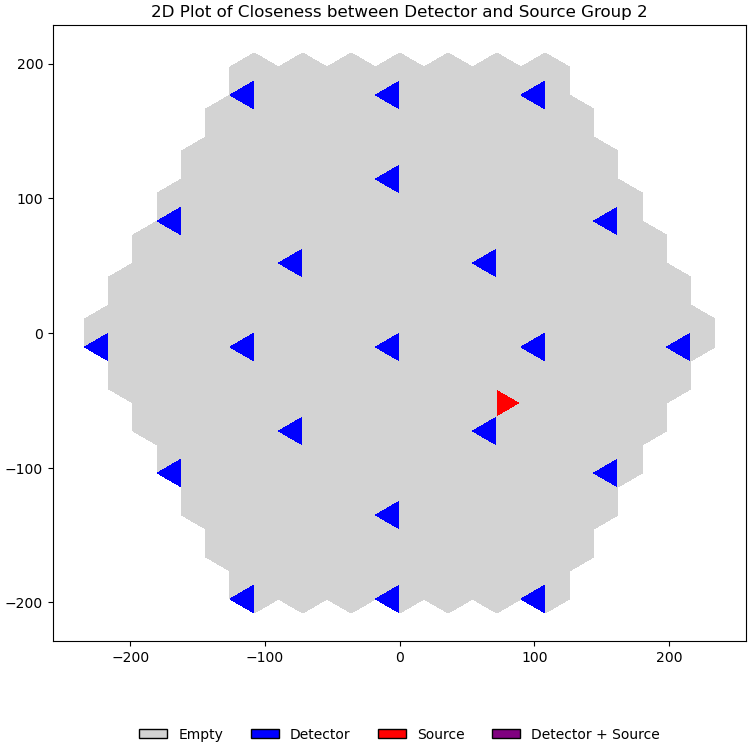
\includegraphics[width=\linewidth]{figures/OBJECTIVES61_TEST_SUITE_2DTriMG_HTTR_level1_iter2_closeness_det_S_categorical_G2.png}
        \end{subfigure}
        \caption{Location of source and detectors in the 2D HTTR case}
        \label{fig:map_S_2DHTTR_AVS1S_back}
\end{figure}

The results of the simulations are described in Table \ref{table:unfold_2DHTTR_AVS1S_back}.
\begin{table}[H]
        \centering
        \caption{Single noise source in 2D HTTR}
        \label{table:unfold_2DHTTR_AVS1S_back}
        \begin{tabular}{ | M{3.5cm} | M{1.5cm} | M{1.5cm} | M{4cm} | M{1.5cm} | } 
         \hline
         \textbf{Method} & \textbf{Energy Group} & \textbf{Hex Number} & \textbf{Neutron Noise Source} ($n/cm^3$) & \textbf{Match?}  \\
         \hline
         Reference & 2 & 42 & $-3.094 \times 10^{-4} + 0.000i$ & --  \\
         \hline
         Backward Elimination & 2 & 42 & $-3.094 \times 10^{-4} + 0.000i$ & Yes  \\
         \hline
        \end{tabular}
\end{table}
The results indicate that the backward elimination method is effective for a single mesh source. This is because the method iterates to find the least number of Green's function combinations that can match the reference.

\subsubsection{Multiple Noise Source}

In this simulation, two-mesh and three-mesh AVS source is unfolded using both the existing and novel methods. For the two-mesh source, the simulation is done with a constant frequency of 10 Hz. Figure \ref{fig:map_S_2DHTTR_AVS2S_back} shows the location of the AVS source.
\begin{figure}[H]
        \centering
        \begin{subfigure}{.48\textwidth}
          \centering
          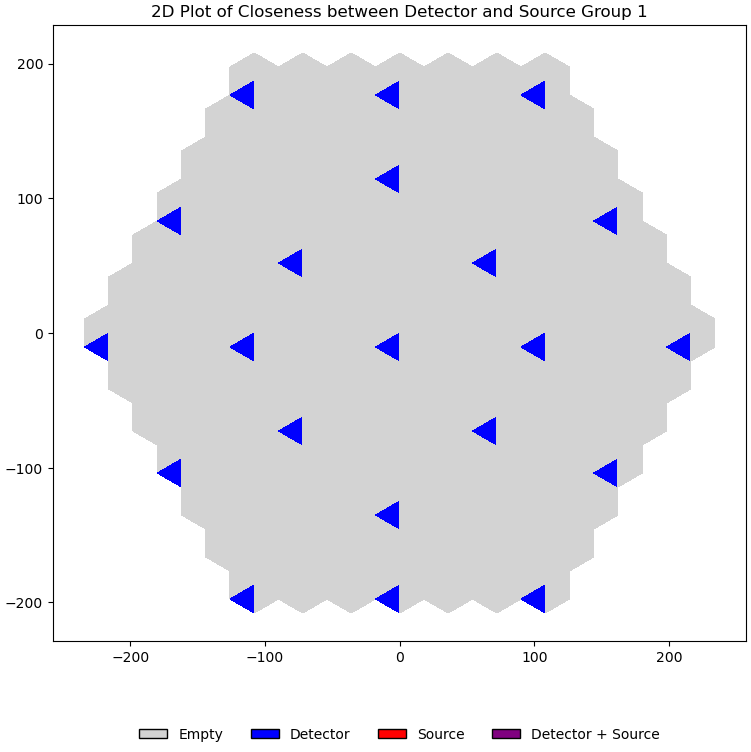
\includegraphics[width=\linewidth]{figures/OBJECTIVES61_TEST_SUITE_2DTriMG_HTTR_level1_iter9_closeness_det_S_categorical_G1.png}
        \end{subfigure}
        \hfill
        \begin{subfigure}{.48\textwidth}
          \centering
          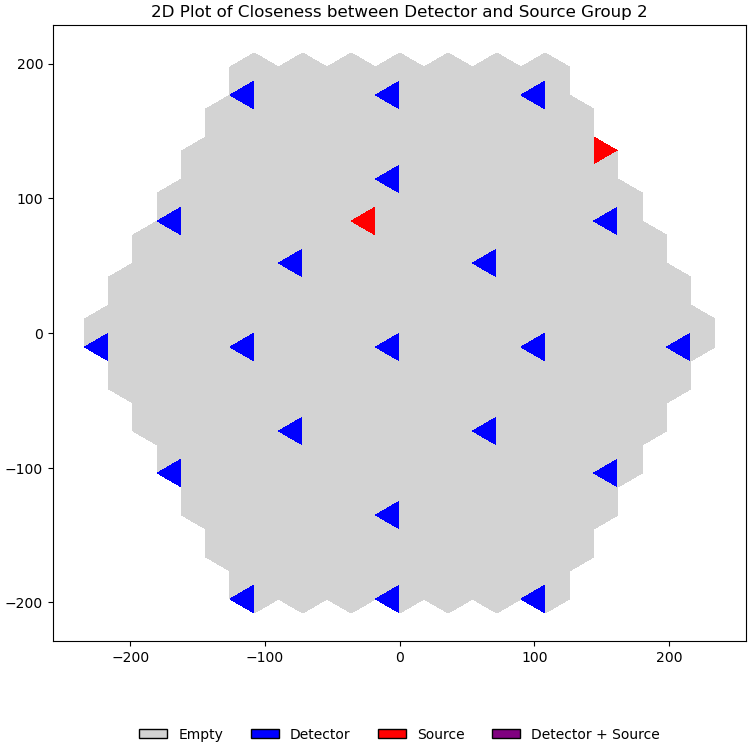
\includegraphics[width=\linewidth]{figures/OBJECTIVES61_TEST_SUITE_2DTriMG_HTTR_level1_iter9_closeness_det_S_categorical_G2.png}
        \end{subfigure}
        \caption{Location of sources and detectors in the 2D HTTR case}
        \label{fig:map_S_2DHTTR_AVS2S_back}
\end{figure}

The results of the simulations are described in Table \ref{table:unfold_2DHTTR_AVS2S_back}.
\begin{table}[H]
        \centering
        \caption{Two noise sources in 2D HTTR}
        \label{table:unfold_2DHTTR_AVS2S_back}
        \begin{tabular}{ | M{3.5cm} | M{1.5cm} | M{1.5cm} | M{4.5cm} | M{1.5cm} | } 
         \hline
         \textbf{Method} & \textbf{Energy Group} & \textbf{Hex Number} & \textbf{Neutron Noise Source} ($n/cm^3$) & \textbf{Match?}  \\
         \hline
         \multirow{2}{*}{Reference} & 2 & 98 & $-1.054 \times 10^{-2}-9.373 \times 10^{-3}j$ & 1  \\
         \cline{2-5}                & 2 & 112 & $-1.739 \times 10^{-4}+0.000i$ & --  \\
         \hline
         \multirow{2}{*}{Backward Elimination} & 2 & 96 & $2.631 \times 10^{-2} - 2.443 \times 10^{-3}i$ & No  \\
         \cline{2-5}                           & 2 & 120 & $-2.598 \times 10^{-2} - 6.998 \times 10^{-5}i$ & No  \\
         \hline
        \end{tabular}
\end{table}

For the three-mesh source, the simulation is done with a constant frequency of 1 Hz. Figure \ref{fig:map_S_2DHTTR_AVS3S_back} shows the location of the AVS source.
\begin{figure}[H]
        \centering
        \begin{subfigure}{.48\textwidth}
          \centering
          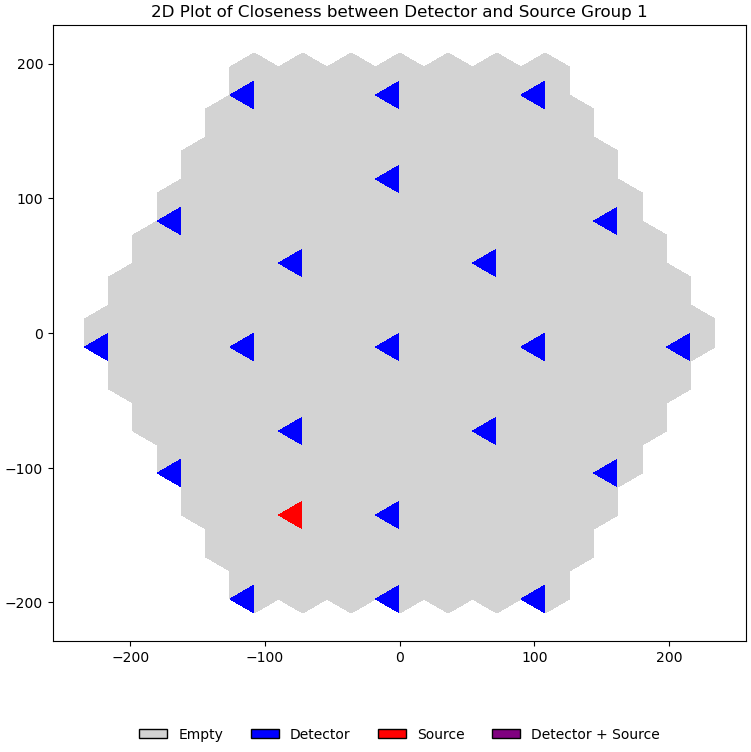
\includegraphics[width=\linewidth]{figures/OBJECTIVES45_TEST10_2DTriMG_HTTR_AVS3S_level1_closeness_det_S_categorical_G1.png}
        \end{subfigure}
        \hfill
        \begin{subfigure}{.48\textwidth}
          \centering
          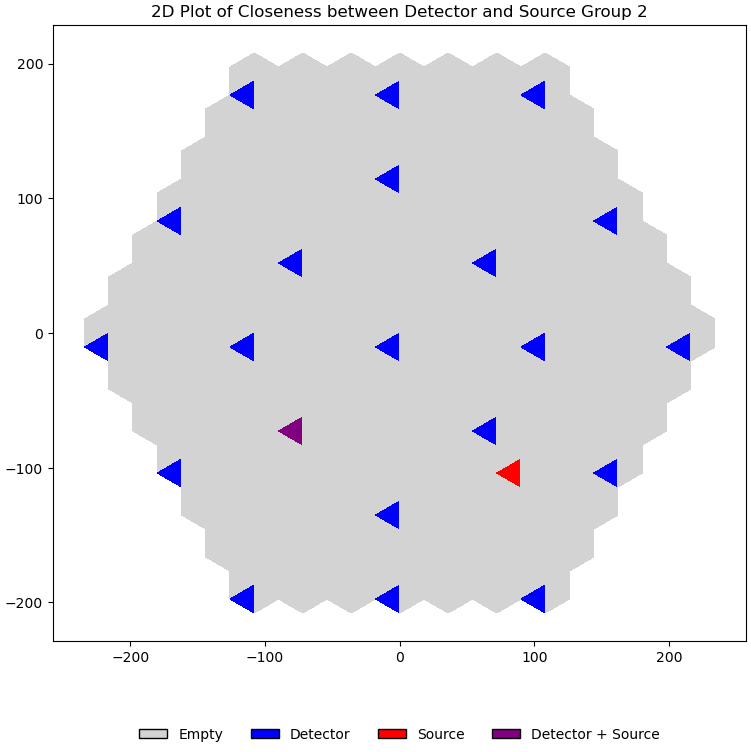
\includegraphics[width=\linewidth]{figures/OBJECTIVES45_TEST10_2DTriMG_HTTR_AVS3S_level1_closeness_det_S_categorical_G2.png}
        \end{subfigure}
        \caption{Location of sources and detectors in the 2D HTTR case}
        \label{fig:map_S_2DHTTR_AVS3S_back}
\end{figure}

The results of the simulations are described in Table \ref{table:unfold_2DHTTR_AVS3S_back}.
\begin{table}[H]
        \centering
        \caption{Three noise sources in 2D HTTR}
        \label{table:unfold_2DHTTR_AVS3S_back}
        \begin{tabular}{ | M{3.5cm} | M{1.5cm} | M{1.5cm} | M{4.5cm} | M{1.5cm} | } 
         \hline
         \textbf{Method} & \textbf{Energy Group} & \textbf{Hex Number} & \textbf{Neutron Noise Source} ($n/cm^3$) & \textbf{Match?}  \\
         \hline
         \multirow{3}{*}{Reference} & 1 & 18 & $-2.797 \times 10^{-8} + 0.000i$ & --  \\
         \cline{2-5}                & 2 & 32 & $-3.341 \times 10^{-6} + 0.000i$ & --  \\
         \cline{2-5}                & 2 & 38 & $-1.053 \times 10^{-4} + 0.000i$ & --  \\
         \hline
         \multirow{3}{*}{Backward Elimination} & 1 & 4 & $-1.178 \times 10^{-1} + 8.899 \times 10^{-4}i$ & No  \\
         \cline{2-5}                           & 2 & 4 & $7.709 \times 10^{-2} - 7.359 \times 10^{-4}i$ & No  \\
         \cline{2-5}                           & 1 & 13 & $6.236 \times 10^{-2} - 4.682 \times 10^{-4}i$ & No  \\
         \hline
        \end{tabular}
\end{table}

The results indicate that the backward elimination method is ineffective in simultaneously unfolding multiple neutron noise sources. This is because during the iteration, it is possible that the Green's functions of the position of the neutron noise source are eliminated. The elimination can happen if, at that combination, the Green's functions that are supposed to be the solution of the problem have small contributions to the solution. This makes the backward elimination method unreliable for unfolding multiple neutron noise sources simultaneously.